% paper/sections/casestudy2.tex — Case Study 2: Tecator (registration, scalar-on-function regression)
% Every number below is a macro written by paper/code/casestudy2.py into
% sections/cs2_numbers.tex (drift gate: paper/code/check_cs_numbers.py).
% Auto-generated by paper/code/casestudy2.py -- do not edit.
% Regenerate: PYTHONPATH=scripts:paper/code python paper/code/casestudy2.py
% Drift gate: PYTHONPATH=scripts:paper/code python paper/code/check_cs_numbers.py
\newcommand{\csTwoNSamples}{240}
\newcommand{\csTwoNChannels}{100}
\newcommand{\csTwoFatMin}{0.9}
\newcommand{\csTwoFatMax}{58.5}
\newcommand{\csTwoNKarcher}{30}
\newcommand{\csTwoKarcherIter}{20}
\newcommand{\csTwoKarcherConverged}{no}
\newcommand{\csTwoNComp}{15}
\newcommand{\csTwoTrainRtwo}{0.974}
\newcommand{\csTwoTrainRtwoRaw}{0.970}
\newcommand{\csTwoCVRtwo}{0.928}
\newcommand{\csTwoCVFolds}{0.934, 0.831, 0.940, 0.971, 0.962}
\newcommand{\csTwoCVRtwoRaw}{0.916}
\newcommand{\csTwoCVRtwoRegRaw}{-0.017}
\newcommand{\csTwoCVRtwoRegDtwo}{0.210}
\newcommand{\csTwoNShown}{30}


\subsection{Registration and Scalar-on-Function Regression: Tecator Data}
\label{subsec:cs2-tecator}

The tecator dataset consists of \csTwoNSamples{} near-infrared absorbance spectra of meat
samples measured at \csTwoNChannels{} spectral channels, with fat content (ranging from
\csTwoFatMin\% to \csTwoFatMax\%) recorded as a scalar response for each sample
\citep{borggaard_thodberg_1992}.  This study pairs two \texttt{fdars}
capabilities---elastic registration under the square-root slope function
(SRSF) framework \citep{srivastava_klassen_2016} and scalar-on-function
functional principal component regression \citep{reiss_ogden_2007}---and uses
the pair to make a methodological point: registration should be applied only
when phase variation is a nuisance, and in near-infrared spectra it is not.

\paragraph{Registration.}
We estimate an elastic Karcher mean from a representative subset of \csTwoNKarcher{} curves
using \texttt{fdars.alignment.karcher\_mean}, with the Fisher--Rao gradient
descent capped at \csTwoKarcherIter{} iterations for speed (it had not met its tolerance when
stopped), and align all \csTwoNSamples{} spectra to that mean with
\texttt{fdars.alignment.align\_to\_target}.  Figure~\ref{fig:cs2-align} shows
the effect: the absorption peak is pulled to a common location across samples.

\paragraph{Scalar-on-function regression.}
Following standard near-infrared practice~\citep{rinnan_2009}, we convert the absorbance curves to
\emph{second-derivative} spectra---B-spline smoothing followed by double
differentiation---which removes additive baseline offsets and linear baseline
slopes (the additive part of light-scatter effects; multiplicative scatter is
not corrected).  Fat content is
then modelled as a linear functional of the second-derivative spectrum via FPC
regression (\texttt{fdars.regression.fregre\_lm}, \csTwoNComp{} components).
Fitting on all \csTwoNSamples{} samples gives a training $R^2 = \csTwoTrainRtwo$
(Figure~\ref{fig:cs2-fit}); the same model on the raw absorbance spectra gives
$R^2 = \csTwoTrainRtwoRaw$.

\paragraph{Cross-validation.}
Five-fold cross-validation of \texttt{FPCRegressor} (\csTwoNComp{} components) via
\texttt{sklearn.\allowbreak model\_selection.\allowbreak cross\_val\_score}
gives a mean $R^2 = \csTwoCVRtwo$ on second-derivative spectra (folds
$[\csTwoCVFolds]$) against $\csTwoCVRtwoRaw$ on the raw spectra---a
small but consistent gain from the preprocessing.

\paragraph{Should the spectra be registered first?}
No.  Repeating the cross-validation on the \emph{registered} spectra drops the
mean $R^2$ to $\csTwoCVRtwoRegRaw$ for the absorbance curves and $\csTwoCVRtwoRegDtwo$ for their second
derivatives.  The positions and shapes of the absorption bands encode the
chemical composition, so the warping that aligns them removes precisely the
information that predicts fat content.  The registration step is therefore
shown as an illustration of the alignment interface, not as preprocessing for
this regression; in applications where timing is a nuisance (such as the
growth-velocity curves in Section~\ref{sec:capabilities}), the same interface
is the right tool.
The complete analysis, including every number above, is reproduced by
\texttt{paper/code/casestudy2.py}.

\begin{figure}[tbp]
  \centering
  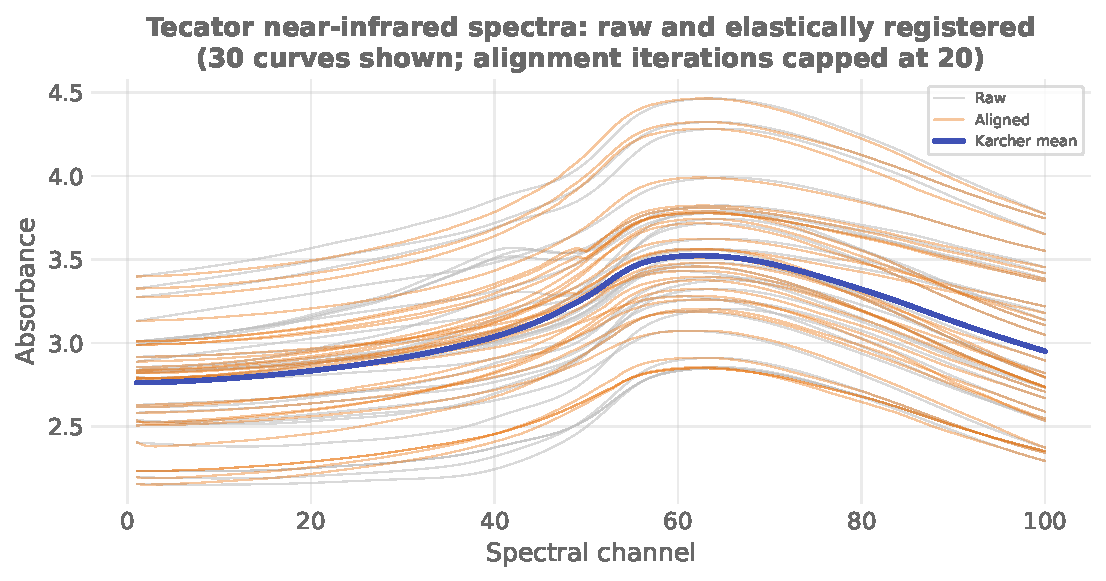
\includegraphics[width=\textwidth]{figures/cs2_tecator_align.pdf}
  \caption{Tecator near-infrared spectra before and after elastic SRSF
    registration (\csTwoNShown{} of \csTwoNSamples{} curves shown).  Grey traces: raw spectra.
    Coloured traces: spectra aligned to the Karcher mean.  Bold trace: the
    estimated Karcher mean used as the registration target (iterations capped
    at \csTwoKarcherIter).  Aligning the absorption peak removes the predictive signal
    (see text).}
  \label{fig:cs2-align}
\end{figure}

\begin{figure}[tbp]
  \centering
  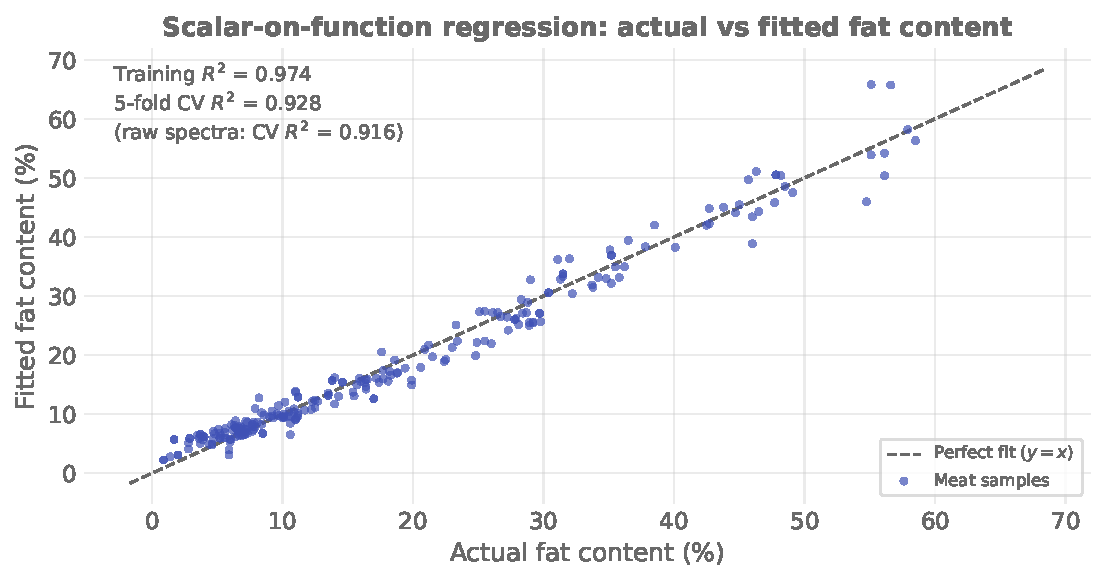
\includegraphics[width=\textwidth]{figures/cs2_tecator_fit.pdf}
  \caption{Scalar-on-function FPC regression on the tecator data: actual
    versus fitted fat content for all \csTwoNSamples{} meat samples, using unregistered
    second-derivative spectra (\texttt{fdars.regression.fregre\_lm},
    \csTwoNComp{} components).  The dashed line marks perfect prediction ($y = x$).
    Training $R^2 = \csTwoTrainRtwo$; 5-fold CV $R^2 = \csTwoCVRtwo$ (raw spectra: $\csTwoCVRtwoRaw$).}
  \label{fig:cs2-fit}
\end{figure}
